\documentclass[../report.tex]{subfiles}
\begin{document}
\graphicspath{{img/}{../img/}}


Since all but one service operations on \textit{ShareIt} are private to clients, and some of these to users, it is important to discuss how access control is handled.

Two consecutive walls will block ones way when reaching \textit{ShareIt}; First a client token validation and secondly a user credential validation. \\

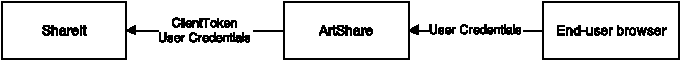
\includegraphics[width=\linewidth]{./AccessControlDeployment.pdf}

\subsection{Token validation}
\label{sec:Token}

The token validation is implemented as a means for \textit{ShareIt} to only allow recognized clients to invoke operations. This works because \textit{ShareIt} and a Client like \textit{ArtShare} share an identical string which we call the clientToken. \textit{ShareIt}'s database has a Client table against which \textit{ShareIt} checks incoming clientTokens. These tokens are static and do not depend on any communication session, but are created specifically for an implementor to use.

In order to associate a token with a client the token has to be transfered through an encrypted channel. However security is not in scope here, which has the consequence that anybody could sniff the token.

Below is the token which \textit{ShareIt} associates with \textit{ArtShare}. The token could be anything digital as long as its' length implicates a brute force attack.

\begin{center}
\texttt{7dac496c534911c0ef47bce1de772502b0d6a6c60b1dbd73c1d3f285f36a0f61}
\end{center}



\subsection{User credential validation}
\label{sec:UserCredential}

Operations on \textit{ShareIt} that need to distinguish a user in any way take a \textit{UserDTO}. In these cases the UserDTO is validated with the database on it's Username and Password properties. An example is the operation to validate whether a User is registered with the system. Here is seen the clientToken argument as discussed in section \ref{sec:Token}. 

\begin{center}
\begin{lstlisting}
	int ValidateUser(UserDTO user, string clientToken);
\end{lstlisting}
\end{center}


While the clientToken has a single purpose, namely to validate clients, the user credential check is multi-functional in the way it determines many types of access rights with the system.


\subsection{Access rights}

\todo{write}


\end{document}